\documentclass[a4paper,11pt]{article}
\usepackage[margin=2cm]{geometry}

\usepackage[nodayofweek]{datetime}
\usepackage{cite}
\usepackage{graphicx}
\longdate

\usepackage{fancyhdr}
\pagestyle{fancyplain}
\fancyhf{}
\lhead{\fancyplain{}{M.Sc.\ Group Project Report}}
\rhead{\fancyplain{}{\today}}
\cfoot{\fancyplain{}{\thepage}}


\title{Implementation of attentional bistability of the dragonfly visual neurons in an intelligent biomimetic agent\\\Large{--- Report One ---}}
\author{Juan Carlos Farah, Panos Almpouras, Ioannis Kasidakis, Erik Grabljevec, Christos Kaplanis\\
       \{jcf214, pa512, ik311, eg1114, ck2714\}@doc.ic.ac.uk\\ \\
       \small{Co-supervisors: Professor Murray Shanahan, Zafeirios Fountas, Pedro Martinez-Mediano}\\
       \small{Course: CO530/533, Imperial College London}
}

\begin{document}
\maketitle

\section{Introduction}

Methods in computer vision have been significantly influenced by the mechanisms of biological insect vision. Our goal in this project is to model the target selection mechanism of the dragonfly and implement it in a biomimetic agent. Dragonflies are notoriously effective at prey capture, making the neural processes that underlie this ability particularly interesting to investigate. 

The centrifugal small ­target motion detector neuron 1 (CSTMD1) is a higher ­order visual neuron in the brain of the dragonfly. This neuron reacts to the presentation of multiple visual stimuli by firing as if only one of the stimuli was present; this is presumably an attentional selection mechanism \cite{w13}. At Professor Shanahan's lab, they have simulated the large contralateral dendritic field of the CSTMD1 neuron with a biophysical multi­compartmental Hodgkin and Huxley model. Along with Klaus Stiefel \cite{ne13}, they found that with certain numbers of inhibitory synapses and potassium conductance densities, two mutually coupled CSTMD1 neurons are capable of a bistable switching process between two input patterns. This bistability can serve as a mechanism for the observed attentional selection.

The high­ level idea of the project is to employ the principle used by the CSTMD1 neuron in a biomimetic agent that behaves like a dragonfly, showing attention-­like target selection when performing a simple foraging task.



\section{Specification}
	\subsection{Goal-Oriented Capture}
	We brainstormed using Goal-Oriented capture in order to determine the requirements for our project. Below is a chart that portrays this process.	
		
	\begin{center}
	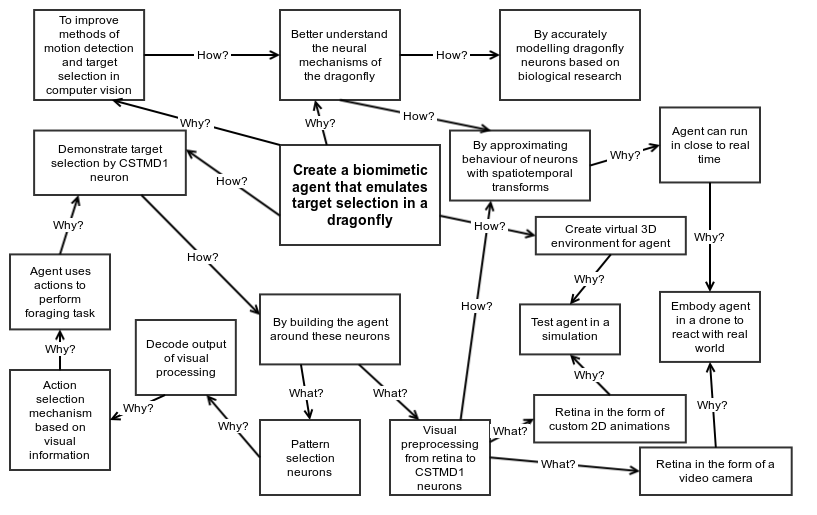
\includegraphics[scale = 0.5]{goalorient}	
	\end{center}

	\subsection{Minimum Requirements (Stage 1)}
	
	The goal-oriented capture enabled us to establish some minimum requirements for the completion of the project. In order to build an agent that can interact with its environment and exhibit the selective function of the CSTMD1 neuron, three main objectives need to be completed:
\begin{enumerate}
	\item (1A) We need to connect the visual input of the agent (in the form 	of either a camera input or a constructed animation) to the modelled CSTMD1 neurons. This will involve:
	\begin{enumerate}
		\item Building a model of the visual processing that occurs between the retina and the actual CSTMD1 neurons of a real dragonfly.
		\item Deciding how many CSTMD1 neurons we will use and how exactly to connect them to the output of our visual pre-processing.
		\item Once connected, test the system for various inputs from simple animations to see if we can recreate the selectivity between two targets observed in actual CSTMD1 neurons. ~\cite{w13}
	\end{enumerate}
	\item (1B) We need to build a layer of pattern recognition neurons that can decode the output of the CSTMD1 neuron.
	\item (1C) We need to integrate the visual processing and the pattern recognition system and add a simple action selection mechanism. For the minimum requirement, we will need two neurons that take input from the pattern recognition system that fire when the dragonfly chooses to go left or right respectively to catch a target.
\end{enumerate} 
 
 	\subsection{Expected implementation (Stage 2)}
 	
 	Beyond the minimum requirements, we expect to enhance the action selection mechanism in order to give a more complex reaction to targets in the visual field . This will involve:
 \begin{enumerate}
 	\item Creating virtual 3D environment for dragonfly agent.
 	\item Enhancing the action selection mechanism to have at least 12 output neurons, giving the dragonfly 12 degrees of motion (6 for rotation and 6 for translation).
 	\item Employing reinforcement learning in the action selection mechanism to train the agent to move more effectively towards the target.
 \end{enumerate}
 
 	\subsection{Possible extensions (Stage3)}
 	
 	Beyond the expected implementation, there are numerous ways we have thought of to extend the project:
 \begin{enumerate}
 	\item Embody the agent in a quadcopter drone (owned by the Neurodynamics lab).
 \end{enumerate}

\section{Another section}

The contents of your report goes here.  Report One should be between 2
and 5 pages, while Report Two should be between 2 and 4 pages
(excluding the appendix).  Reports should be typed in Latex, using an
11-point font size, with 2cm margins all around, and spaced normally.
Please use this template as a starting point.

The contents of your report goes here.  Report One should be between 2
and 5 pages, while Report Two should be between 2 and 4 pages
(excluding the appendix).  Reports should be typed in Latex, using an
11-point font size, with 2cm margins all around, and spaced normally.
Please use this template as a starting point.

The contents of your report goes here.  Report One should be between 2
and 5 pages, while Report Two should be between 2 and 4 pages
(excluding the appendix).  Reports should be typed in Latex, using an
11-point font size, with 2cm margins all around, and spaced normally.
Please use this template as a starting point.


%%%%%%%%%%%%%%%%%%%%%%%%%%%%%%%%%%%%%%%%%%%%%%%%%%%%%%%%%%%%

\section{Work Allocation}

%%%%%%%%%%%%%%%%%%%%%%%%%%%%%%%%%%%%%%%%%%%%%%%%%%%%%%%%%%%%

\subsection{Organisation}


Juan Carlos Farah was selected to become Group Leader, due his experiece in organisation and software development.

He took responsibility for project coordination and code integration.


Our project is split in two stages. Stage one and two. We are allocating team members on rolling basis, however in

stage one our team is split in two sub-groups. One sub-group is working on action selection, while other is working

on dragonfly neurons. We assigned members according to estimation of how long each part will take.


The table below shows how we have allocated work so far:


\begin{table}[ht]

\centering % used for centering table

\begin{tabular}{l c c c c c} % centered columns (4 columns)

%inserts double horizontal lines

& Leader & Stage 1A & Stage 1B & Stage 2 & Stage 3\\ [0.5ex] % inserts table

%heading

\hline % inserts single horizontal line

Juan Carlos Farah & x & & x & x & x \\ % inserting body of the table

Erik Grabljevec & & x & & x & x \\

Christos Kaplanis & & x & & x & x \\

Panagiotis Almpouras & & & x & x & x \\

Ioannis Kasidakis & & x & & x & x \\ [1ex] % [1ex] adds vertical space

\end{tabular}

\label{table:nonlin} % is used to refer this table in the text

\end{table}


%%%%%%%%%%%%%%%%%%%%%%%%%%%%%%%%%%%%%%%%%%%%%%%%%%%%%%%%%%%%


\section{And maybe another one}

The contents of your report goes here.  Report One should be between 2
and 5 pages, while Report Two should be between 2 and 4 pages
(excluding the appendix).  Reports should be typed in Latex, using an
11-point font size, with 2cm margins all around, and spaced normally.
Please use this template as a starting point.

The contents of your report goes here.  Report One should be between 2
and 5 pages, while Report Two should be between 2 and 4 pages
(excluding the appendix).  Reports should be typed in Latex, using an
11-point font size, with 2cm margins all around, and spaced normally.
Please use this template as a starting point.

The contents of your report goes here.  Report One should be between 2
and 5 pages, while Report Two should be between 2 and 4 pages
(excluding the appendix).  Reports should be typed in Latex, using an
11-point font size, with 2cm margins all around, and spaced normally.
Please use this template as a starting point.


\section{Final section}

The contents of your report goes here.  Report One should be between 2
and 5 pages, while Report Two should be between 2 and 4 pages
(excluding the appendix).  Reports should be typed in Latex, using an
11-point font size, with 2cm margins all around, and spaced normally.
Please use this template as a starting point.

The contents of your report goes here.  Report One should be between 2
and 5 pages, while Report Two should be between 2 and 4 pages
(excluding the appendix).  Reports should be typed in Latex, using an
11-point font size, with 2cm margins all around, and spaced normally.
Please use this template as a starting point.

The contents of your report goes here.  Report One should be between 2
and 5 pages, while Report Two should be between 2 and 4 pages
(excluding the appendix).  Reports should be typed in Latex, using an
11-point font size, with 2cm margins all around, and spaced normally.
Please use this template as a starting point.

\bibliography{report1}{}
\bibliographystyle{plain}



\end{document}

